% ==============================================================================
% CAPÍTULO 3 - MODELAGEM MATEMÁTICA DO SUBSISTEMA ELÉTRICO E DE ARMAZENAMENTO
% Arquivo: elementos/05_capitulo3.tex
% ==============================================================================

\section{MODELAGEM MATEMÁTICA DO SUBSISTEMA ELÉTRICO E DE ARMAZENAMENTO}
\label{sec:capitulo3}

\subsection{Premissas de Rendimento Estático e Dinâmico}
\label{sec:premissas-eta}

O dimensionamento elétrico parte das premissas de rendimento estático e dinâmico consolidadas nesta seção. A distribuição primária adota barramento HVDC regulado para minimizar as perdas ôhmicas por condução, em estrita aderência às diretrizes de veículos espaciais da NASA \cite{bever2006hvguide,ferguson2006nasastd4005,kerslake2011septug,sarfi2024mwscale,nasa2026smallspacecraft}.

\subsection{Arquitetura Geral de Potência e Distribuição Primária}
\label{sec:distribuicao-primaria}
\label{sec:arquitetura_barramento_balanco}

A topologia de distribuição primária de alta tensão é ilustrada na Figura~\ref{fig:hvdc}, fundamentada na arquitetura de distribuição proposta por Sarfi e Beik \cite{sarfi2024mwscale}, na qual a geração primária alimenta um barramento central regulado em $V_{bus} = 400\text{ V}$.

\begin{figure}[htbp]
    \centering
    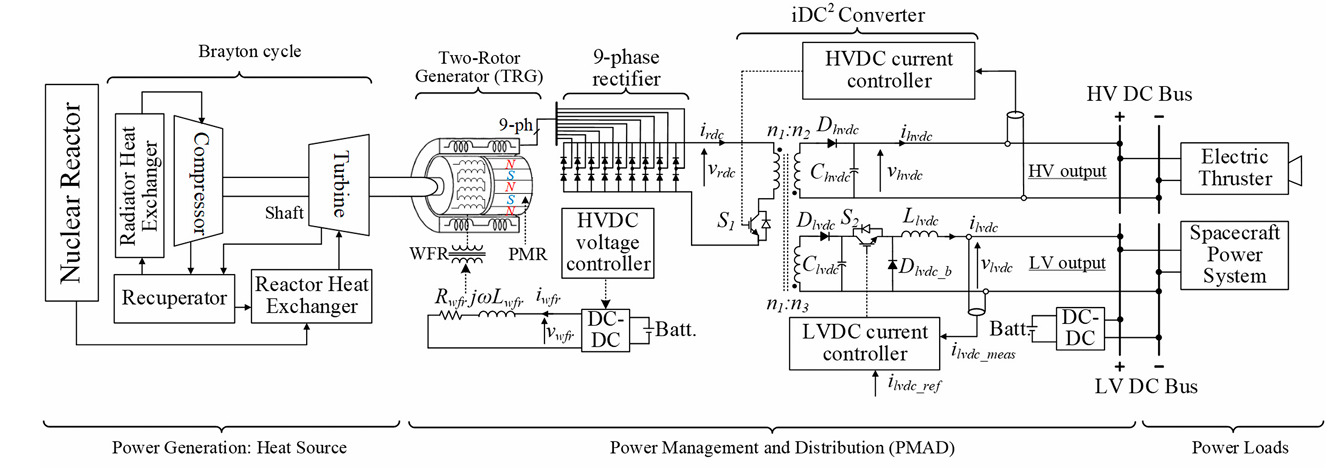
\includegraphics[width=0.85\textwidth]{figuras/figura_3_1_1_arquitetura_HVDC.png}
    \caption{Arquitetura conceitual de barramento de alta tensão e distribuição de potência.}
    \label{fig:hvdc}
    \vspace{2pt}\par\noindent{\footnotesize Fonte: adaptado de Sarfi e Beik \cite{sarfi2024mwscale}.}
\end{figure}

As eficiências dos conversores chaveados e as referências tecnológicas de semicondutores espaciais são sumarizadas na Tabela~\ref{tab:eta-ref}.

\begin{table}[htbp]
\centering
\small
\caption{Valores nominais e referências tecnológicas para os estágios de conversão.}
\label{tab:eta-ref}
\begin{tabular}{p{3.2cm} p{2.8cm} p{6.8cm}}
\toprule
\textbf{Referência} & \textbf{Estágio} & \textbf{Informação Utilizada} \\
\midrule
TPS50601A-SP \cite{ti_tps50601a} & Buck síncrono rad-hard, 3--7~V & Rendimento de pico de 96,6\%; base do modelo descendente. \\
ISL70003SEH \cite{renesas_isl70003seh} & Buck síncrono rad-hard, 3--13,2~V & Pico de 95\%; curvas de rendimento sob variação térmica. \\
RIC70849F \cite{infineon_ric70849f} & Controlador Buck GaN & Define a classe tecnológica de chaveamento a 150~kHz. \\
Huselstein et al. \cite{huselstein2024} & DAB isolado (BOOST-DAB), 30~kW & Rendimento nominal de aproximadamente 97\%. \\
UM3198 \cite{st_um3198} & DAB bidirecional SiC, 25~kW & Rendimento de pico de 98,2\% em 100~kHz. \\
Esteve et al. \cite{esteve2024} & DAB com modulação SPS & Estratégia de modulação com frequência variável. \\
\bottomrule
\end{tabular}
\vspace{2pt}\par\noindent{\footnotesize Fonte: elaborado pelo autor a partir dos documentos citados.}
\end{table}

A seleção dos semicondutores e componentes magnéticos dos conversores estáticos é detalhada na Seção~\ref{sec:gan-dcdc} (com propriedades do material de núcleo magnético de alta frequência consolidada na Tabela~\ref{tab:anexo_ferroxcube_3c95} do Anexo~A). Os requisitos de isolamento dielétrico, espaçamento em placa e imunidade a descargas por efeito corona e arco elétrico em plasma de baixa órbita (LEO) foram balizados segundo normas consolidadas da NASA e da ESA \cite{nasa2026smallspacecraft,ECSS_E_ST_31C_2008,kerslake2011septug,bever2006hvguide,ferguson2006nasastd4005}. As diretrizes para os ensaios térmicos e ciclos de vida útil do sistema de baterias de íons de lítio seguem as recomendações de engenharia aeroespacial \cite{nasa2021liionguidelines,jun2020leobattery}.

\subsection{Estabilidade de Pequenos Sinais e Critério de Middlebrook}
\label{sec:estabilidade-middlebrook}

A impedância incremental refletida pelas cargas computacionais sob regulação em ponto de carga ($P_{CPL}$) e o critério clássico de estabilidade de Middlebrook \cite{middlebrook1976} impõem limites conservadores de impedância de saída para garantir amortecimento supercrítico ($\zeta \ge 1$). Nos barramentos primário e secundário, a impedância de saída passiva da rede é governada por:
\begin{equation}
    Z_{out}(s) = \frac{(s L_{dist} + R_{dist})(s C_{bus} ESR + 1)}{s^2 L_{dist} C_{bus} + s C_{bus} (R_{dist} + ESR) + 1}
    \label{eq:zout_bus}
\end{equation}
\begin{equation}
    C_{bus,min} \ge \max\left( \frac{4 L_{dist}}{R_{dist}^2}, \, \frac{L_{dist} \Delta I^2}{V_{nom}^2 - V_{min}^2}, \, \frac{L_{dist} P_{CPL}^2 \cdot GM^2}{V_{bus}^4} \right)
    \label{eq:cbus}
\end{equation}

Para o barramento primário de $400\text{ V}$ operando com carga constante de $20\text{ kW}$, tem-se:
\begin{align}
    |r_{in,400V}| &= \frac{V_{bus}^2}{P_{CPL}} = \frac{400^2}{20\times 10^3} = 8{,}00\,\Omega \\
    |Z_{out,400}| &\le 0{,}1 \cdot |r_{in,400V}| = 0{,}800\,\Omega
\end{align}
mantendo uma margem de segurança estritamente superior ao teto exigido por projeto.

\subsection{Subsistema de Armazenamento Eletroquímico (BESS)}
\label{sec:bess}
\label{sec:bess-orbital}

A Figura~\ref{fig:bess-orbital} ilustra o comportamento dinâmico de carga e descarga do banco de baterias BESS ao longo de múltiplos ciclos orbitais em baixa órbita terrestre, considerando a carga base contínua $P_{base}$.

\begin{figure}[htbp]
    \centering
    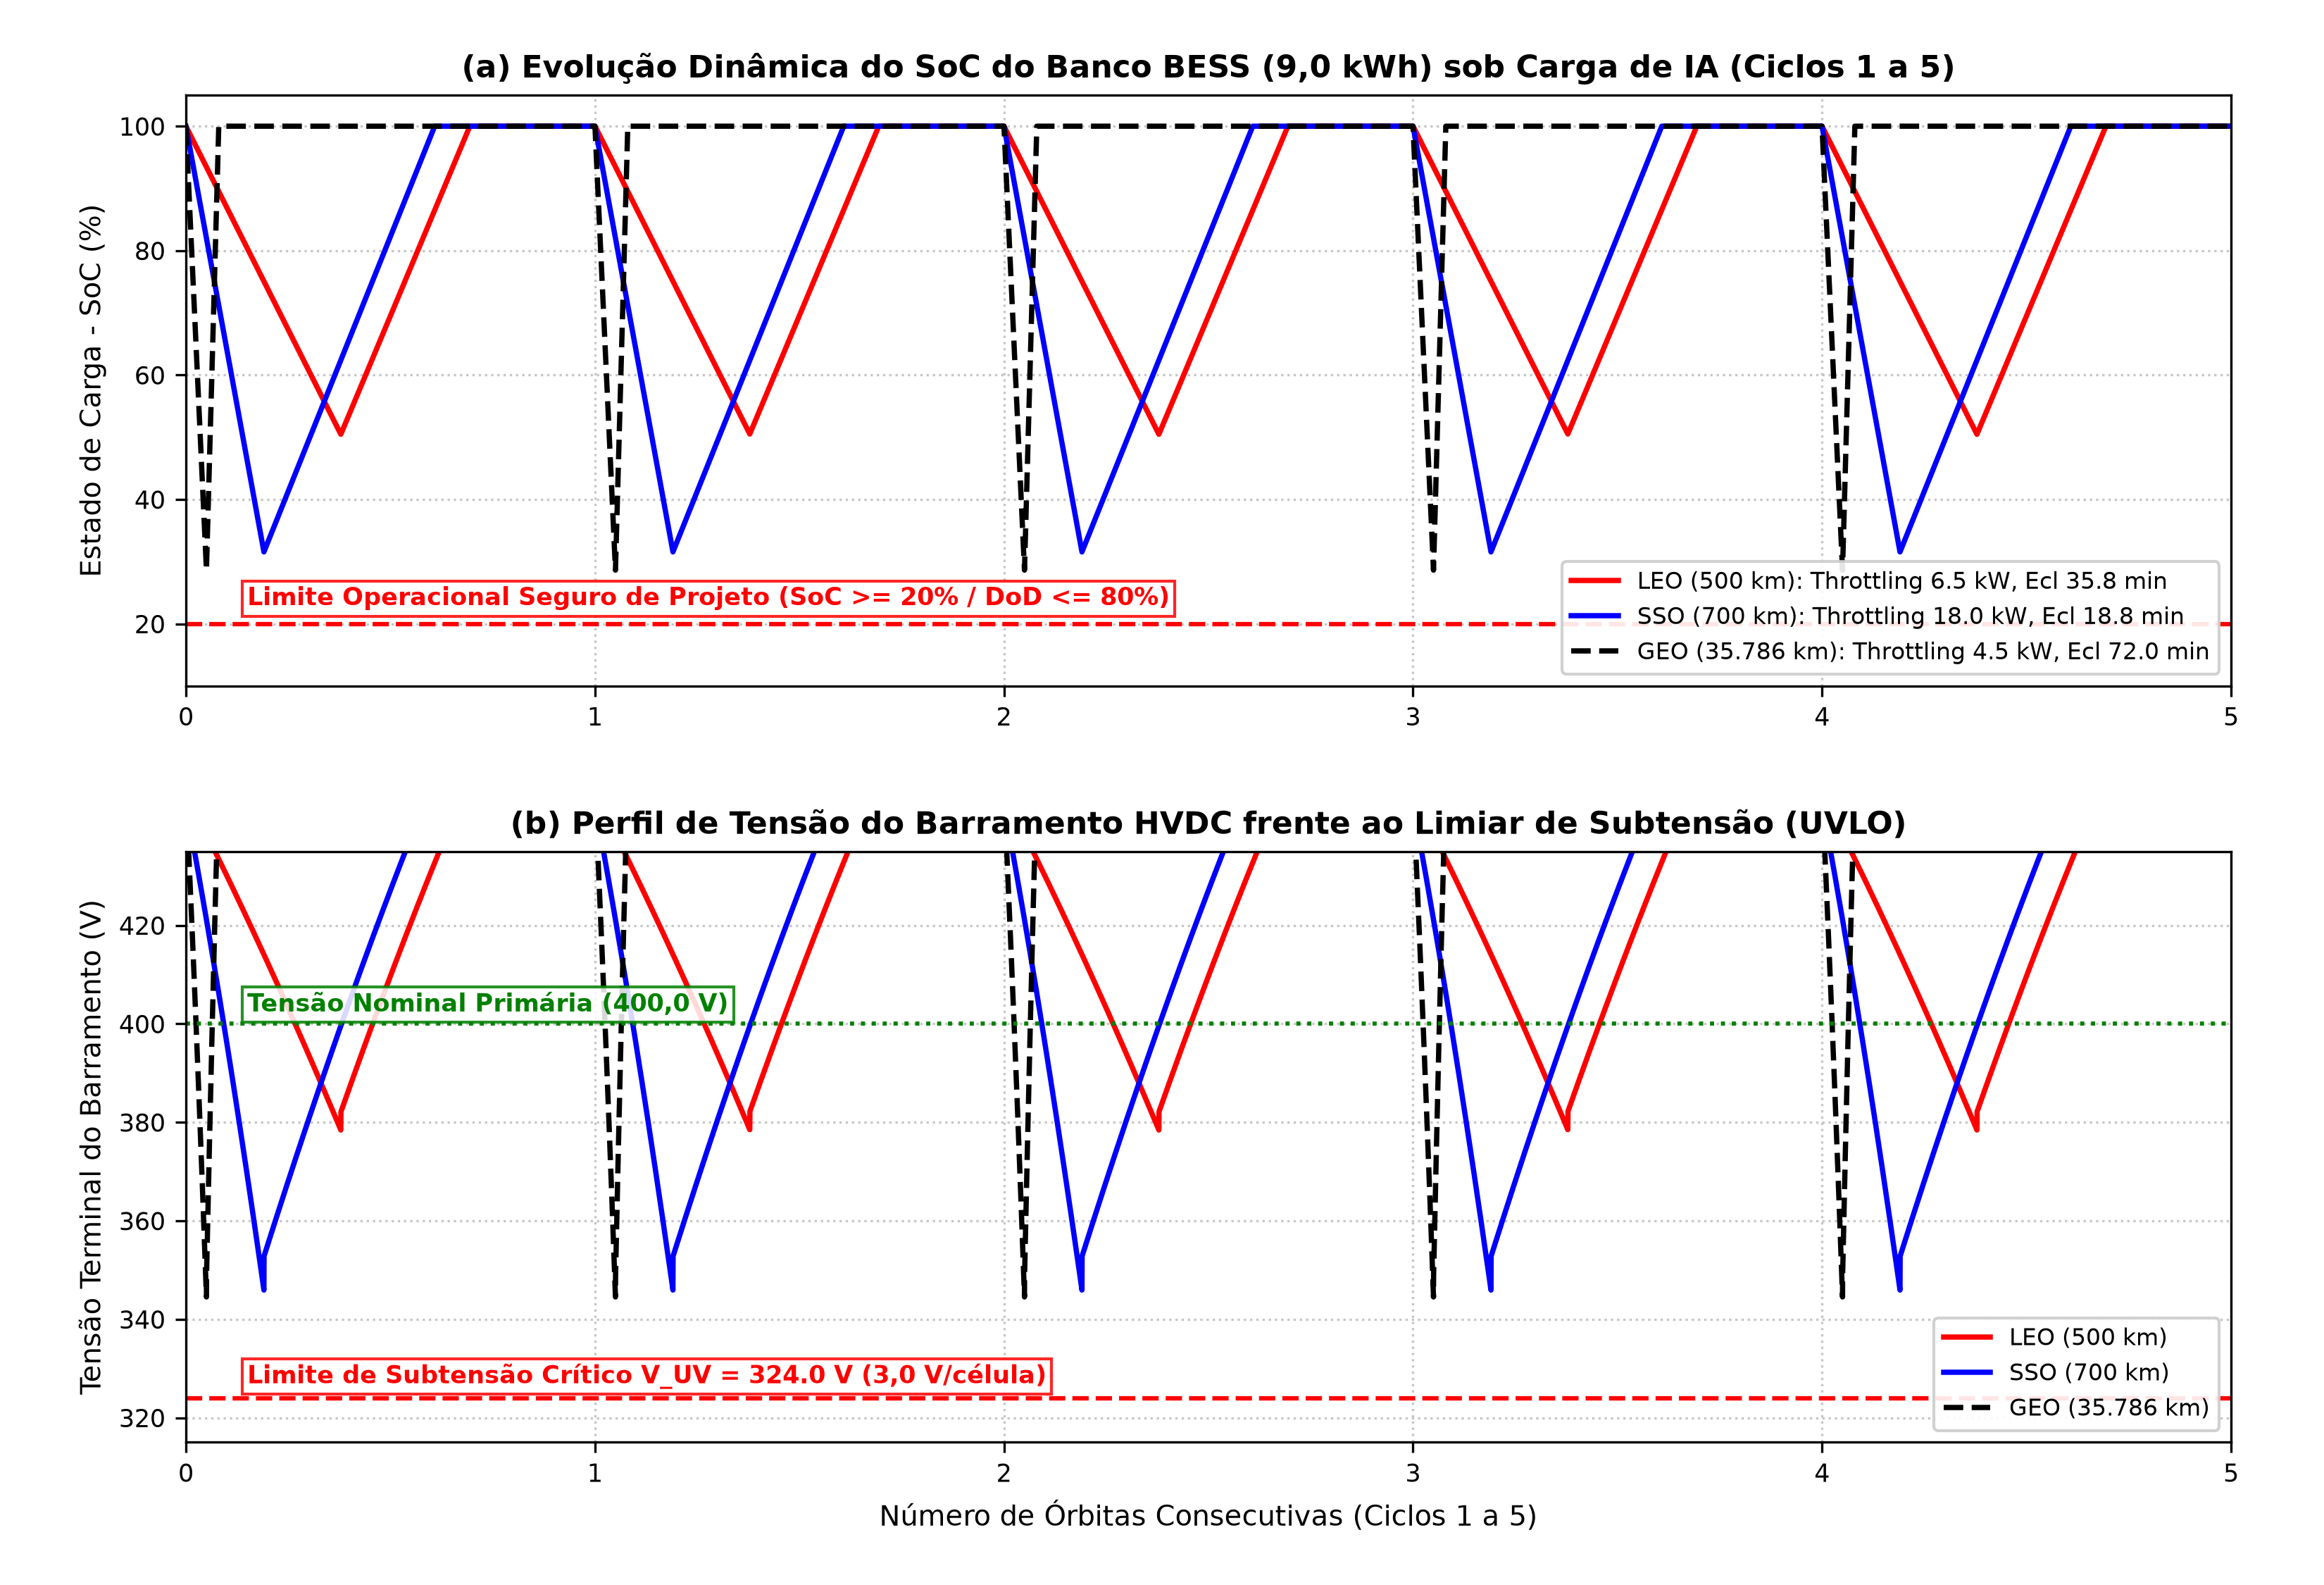
\includegraphics[width=0.90\textwidth]{figuras/figura_3_1_balanco_orbital_bess.png}
    \caption{Balanço orbital de energia e evolução do estado de carga (SoC) do BESS.}
    \label{fig:bess-orbital}
    \vspace{2pt}\par\noindent{\footnotesize Fonte: elaborado pelo autor.}
\end{figure}

A gestão operacional do subsistema de armazenamento é classificada em três regimes:
\begin{enumerate}[label=\textbf{\alph*.)}, leftmargin=1.5cm]
    \item \textbf{Modo de Falha BAT-F01 (Falha do TEMS / Sobrecarga sem Modulação):} Na ausência de redução da carga de processamento das GPUs durante a umbra da Terra, o banco opera em descarga profunda acelerada, reduzindo drasticamente a retenção de capacidade cíclica da bateria.
    \item \textbf{Regime Nominal com Modulação de Carga (Controle TEMS):} Modulação adaptativa das cargas de computação via técnicas de DVFS ao longo do eclipse, mantendo a profundidade de descarga ($\mathrm{DoD}$) estritamente dentro da faixa recomendada de $20\%$ a $30\%$, em conformidade com a norma ECSS-E-ST-20-32C.
    \item \textbf{Recarga Solar e Proteção por Controle CC-CV:} Durante o período de insolação, a taxa de recarga solar é regulada em corrente constante (CC) até atingir a tensão de corte de flutuação, migrando suavemente para tensão constante (CV).
\end{enumerate}

O comportamento estatístico do banco de baterias ao longo de 20 órbitas é detalhado na Tabela~\ref{tab:bess20}.

\begin{table}[htbp]
\centering
\small
\caption{Avaliação do BESS ao longo de 20 órbitas sob diferentes regimes e órbitas.}
\label{tab:bess20}
\begin{tabular}{p{3.6cm} p{1.9cm} r r r r p{2.4cm}}
\toprule
\textbf{Caso} & \textbf{Regime} & \textbf{$P_{IT}$ sol} & \textbf{$P_{pv}$} & \textbf{$SoC_{min}$} & \textbf{$V_{min}$} & \textbf{Status} \\
 & & \textbf{(kW)} & \textbf{(kW)} & \textbf{(\%)} & \textbf{(V)} & \\
\midrule
nominal\_32kW\_script & LEO 500 km & 32,00 & 44,45 & 45,97 & 375,83 & OK \\
nominal\_40kW\_cap4 & LEO 500 km & 40,00 & 44,45 & 0,00 & $<324$ & VIOLA (3ª órbita) \\
nominal\_Pmax\_sust & LEO 500 km & 37,99 & 46,14 & 45,58 & 375,32 & OK \\
falha\_BAT\_F01 & LEO 500 km & 40,00 & 44,45 & 0,00 & $<324$ & VIOLA ($t\approx19{,}4$~min) \\
nominal\_32kW\_script & SSO 700 km & 32,00 & 44,45 & 28,08 & 351,13 & OK \\
nominal\_40kW\_cap4 & SSO 700 km & 40,00 & 44,45 & 0,00 & $<324$ & VIOLA (2ª órbita) \\
nominal\_Pmax\_sust & SSO 700 km & 38,10 & 46,14 & 27,75 & 350,66 & OK \\
falha\_BAT\_F01 & SSO 700 km & 40,00 & 44,45 & 0,00 & $<324$ & VIOLA ($t\approx108{,}1$~min) \\
nominal\_32kW\_script & GEO & 32,00 & 44,45 & 20,42 & 346,14 & OK \\
nominal\_40kW\_cap4 & GEO & 40,00 & 44,45 & 20,42 & 346,14 & OK \\
nominal\_Pmax\_sust & GEO & 40,00 & 46,14 & 20,42 & 346,14 & OK \\
falha\_BAT\_F01 & GEO & 40,00 & 44,45 & 0,00 & $<324$ & VIOLA ($t\approx19{,}5$~min) \\
\bottomrule
\end{tabular}
\vspace{2pt}\par\noindent{\footnotesize Fonte: elaborado pelo autor (Script~3.1, Apêndice~B).}
\end{table}

A potência máxima sustentável de processamento de dados ($P_{IT,max}$) frente à capacidade fotovoltaica da asa solar é confrontada na Tabela~\ref{tab:pitmax}.

\begin{table}[htbp]
\centering
\small
\caption{Capacidade de potência máxima de TI sustentável em fim de vida (EOL).}
\label{tab:pitmax}
\begin{tabular}{p{2.2cm} p{4.2cm} r r r}
\toprule
\textbf{Regime} & \textbf{Cenário Fotovoltaico EOL} & \textbf{$P_{pv}$ (kW)} & \textbf{$P_{IT,max}$ (kW)} & \textbf{Folga (kW)} \\
\midrule
LEO 500 km & 85$^\circ$C (clamp 444,4 V) & 46,14 & 37,99 & $-2{,}01$ \\
LEO 500 km & 65$^\circ$C ($V_{bus}=400$ V) & 49,73 & 40,00 & 0,00 \\
LEO 500 km & 28$^\circ$C (3 diodos) & 54,18 & 40,00 & 0,00 \\
SSO 700 km & 85$^\circ$C (clamp 444,4 V) & 46,14 & 38,10 & $-1{,}90$ \\
SSO 700 km & 65$^\circ$C ($V_{bus}=400$ V) & 49,73 & 40,00 & 0,00 \\
SSO 700 km & 28$^\circ$C (3 diodos) & 54,18 & 40,00 & 0,00 \\
GEO & 85$^\circ$C (clamp 444,4 V) & 46,14 & 40,00 & 0,00 \\
GEO & 65$^\circ$C ($V_{bus}=400$ V) & 49,73 & 40,00 & 0,00 \\
GEO & 28$^\circ$C (3 diodos) & 54,18 & 40,00 & 0,00 \\
\bottomrule
\end{tabular}
\vspace{2pt}\par\noindent{\footnotesize Fonte: elaborado pelo autor. Todos os cenários atendem a 20 órbitas completas.}
\end{table}

Durante a passagem pelo cone de sombra da Terra, a perda de potência dissipada por efeito Joule no pack eletroquímico é deduzida de forma desmembrada por:
\begin{equation}
\begin{split}
    \bar{P}_{J} &= R_{0} \cdot \bar{I}_{ecl}^2 = R_{0} \left( \frac{P_{base}}{\bar{V}_{bat}} \right)^2 \\
                &= 45\times 10^{-3} \times \left( \frac{1000}{375{,}83} \right)^2 \approx 0{,}319\,\mathrm{W/pack} \implies \bar{P}_{J,tot} = 58{,}3\,\mathrm{W}
\end{split}
\label{eq:perda_joule_bess}
\end{equation}

\subsection{Proteção de Alta Tensão e Chaves de Estado Sólido (SSPC)}
\label{sec:sspc}

A atuação do controlador de potência de estado sólido (SSPC) sob evento de curto-circuito franco no barramento primário é apresentada na Figura~\ref{fig:curto}.

\begin{figure}[htbp]
    \centering
    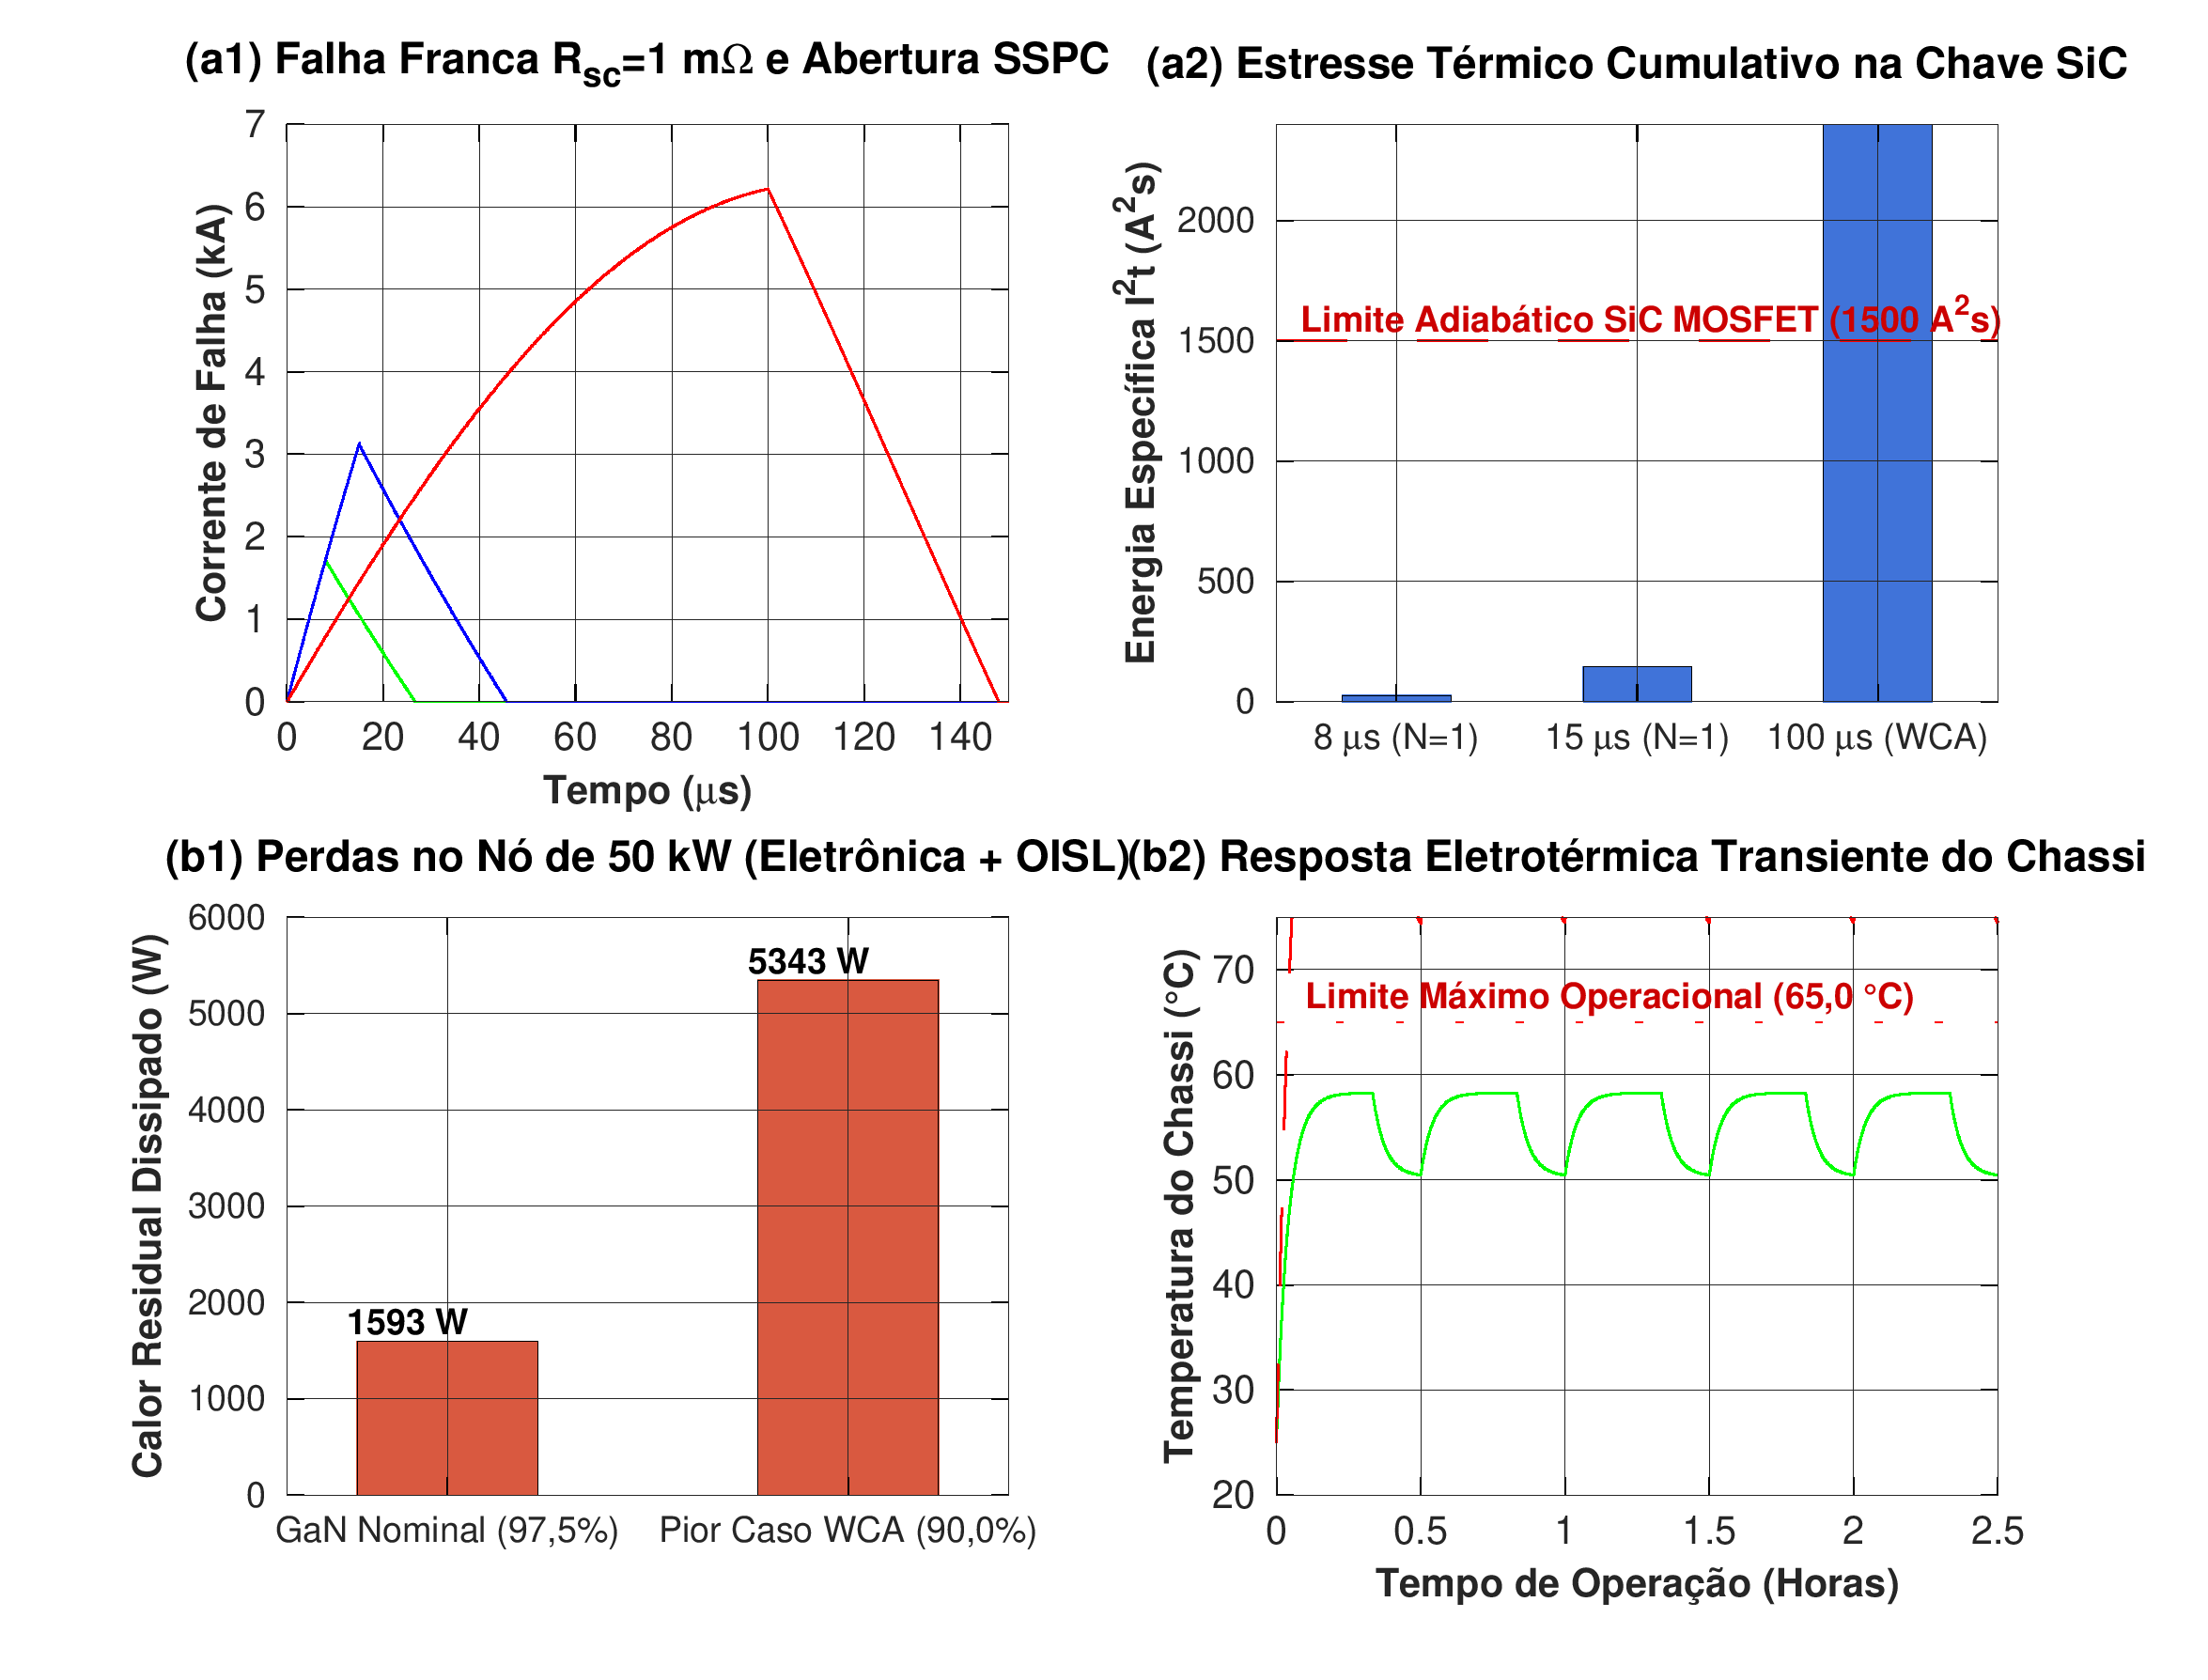
\includegraphics[width=0.85\textwidth]{figuras/figura_3_2_falhas_eletrotermicas_sspc.png}
    \caption{Resposta transitória de extinção de falta e sobretensão induzida no SSPC.}
    \label{fig:curto}
    \vspace{2pt}\par\noindent{\footnotesize Fonte: elaborado pelo autor.}
\end{figure}

O comportamento térmico e a taxa de quebra de corrente $di/dt$ obedecem às limitações físicas impostas pela susceptibilidade radiativa dos semicondutores de potência \cite{galloway2018,lauenstein2018}. O balanço térmico do chassi e dos dissipadores de calor em regime contínuo e transitório é reportado na Tabela~\ref{tab:chassi}.

\begin{table}[htbp]
\centering
\small
\caption{Diagnóstico de perdas e temperatura máxima do estágio conversor.}
\label{tab:chassi}
\begin{tabular}{p{2.2cm} r r r r r r p{1.4cm}}
\toprule
\textbf{Caso Térmico} & \textbf{$\eta_{dab}$} & \textbf{$G_{th}$} & \textbf{$T_{sink}$} & \textbf{$P_{loss}$} & \textbf{$T_{max}$} & \textbf{Margem} & \textbf{Status} \\
 & \textbf{(\%)} & \textbf{(W/K)} & \textbf{($^\circ$C)} & \textbf{(W)} & \textbf{($^\circ$C)} & \textbf{vs. 65$^\circ$C} & \\
\midrule
nominal & 95,0 & 120,0 & 45,00 & 2843,2 & 68,69 & $-3{,}69$ & VIOLA \\
falha\_WCA & 90,0 & 80,0 & 45,00 & 5343,2 & 111,63 & $-46{,}63$ & VIOLA \\
nominal & 95,0 & 120,0 & 51,94 & 2843,2 & 75,63 & $-10{,}63$ & VIOLA \\
falha\_WCA & 90,0 & 80,0 & 51,94 & 5343,2 & 118,57 & $-53{,}57$ & VIOLA \\
nominal & 95,0 & 120,0 & 55,00 & 2843,2 & 78,69 & $-13{,}69$ & VIOLA \\
falha\_WCA & 90,0 & 80,0 & 55,00 & 5343,2 & 121,63 & $-56{,}63$ & VIOLA \\
\bottomrule
\end{tabular}
\vspace{2pt}\par\noindent{\footnotesize Fonte: elaborado pelo autor (Script~3.1, integração em 2,5~h).}
\end{table}

A Tabela~\ref{tab:wca-hvdc} sintetiza os parâmetros limites de projeto e condições de pior caso (\textit{Worst-Case Analysis} --- WCA) para o barramento HVDC.

\begin{table}[htbp]
\centering
\small
\caption{Parâmetros de projeto e limites operacionais para o barramento HVDC.}
\label{tab:wca-hvdc}
\begin{tabular}{p{3.2cm} p{1.2cm} p{1.8cm} p{2.2cm} p{1.8cm} p{3.2cm}}
\toprule
\textbf{Parâmetro} & \textbf{Símb.} & \textbf{Mínimo} & \textbf{Nominal} & \textbf{Máximo} & \textbf{Referência / Origem} \\
\midrule
Tensão do barramento & $V_{bus}$ & 324,0 V & 400,0 V & 442,8 V & \cite{bever2006hvguide,ferguson2006nasastd4005,nasa2026smallspacecraft} \\
Potência demandada & $P_{load}$ & 3,0 kW & 42,24 kW & 50,0 kW & 2 racks IA, perdas e bus \\
Rendimento do DAB & $\eta_{dab}$ & 90,0\% & 95,0\% & 96,55\% & \cite{huselstein2024,st_um3198} \\
Rendimento do Buck & $\eta_{buck}$ & --- & 91,0\% & 96,6\% & \cite{ti_tps50601a,renesas_isl70003seh} \\
Carga em eclipse & $P_{base}$ & --- & 1,00 kW & --- & Hipótese de projeto \\
BESS ($E_{bat}, R_0$) & Pack & 8,4 kWh / 32~m$\Omega$ & 9,0 kWh / 45~m$\Omega$ & 9,6 kWh / 85~m$\Omega$ & Células espaciais Li-ion \\
Resistência de linha & $R_{dist}$ & 10 m$\Omega$ & 14 m$\Omega$ & 50 m$\Omega$ & Barramento alumínio AWG 4 \\
Amortecimento & $\zeta$ & 0,097 & 0,358 & 0,484 & Rede passiva com ESR \\
Indutância e capacit. & $L, C$ & 1,0 $\mu$H / 1,5 mF & 1,8 $\mu$H / 4,7 mF & 4,0 $\mu$H / 6,0 mF & Desacoplamento HVDC \\
Tempo de corte SSPC & $t_{trip}$ & 8 $\mu$s & 15 $\mu$s & 74,54 $\mu$s & Limiar adiabático GaN \\
Religamento de falta & $N_{rel}$ & 0 & --- & 0 & Latch-off definitivo \\
Condutância ao LHP & $G_{th}$ & 80 W/K & 120 W/K & 160 W/K & \cite{gilmore2002handbook,meseguer2012thermal} \\
\bottomrule
\end{tabular}
\vspace{2pt}\par\noindent{\footnotesize Fonte: elaborado pelo autor.}
\end{table}

\subsection{Modelagem do Gerador Fotovoltaico Multijunção e Rastreamento MPPT}
\label{sec:fv}

O número de strings em paralelo necessárias para suprir a demanda da carga de pico no barramento regulado é governado pela relação de dimensionamento:
\begin{equation}
    N_{p,req} = \left\lceil \frac{P_{bus,alvo}}{N_s \cdot P_{mpp,cel} \cdot \eta_{buck}} \right\rceil
\end{equation}

Para o nó de $50\text{ kW}$ em início de vida (BOL), a potência instalada e a tensão de máxima potência da string sob temperatura de catálogo ($28^\circ\text{C}$) são expressas por:
\begin{align}
    P_{BOL} &= 52.416 \times (2{,}406\text{ V} \times 0{,}5282\text{ A}) \approx 66{,}61\,\mathrm{kW} \\
    V_{mp,str}(+28^\circ\mathrm{C}) &= 208 \times 2{,}406\,\mathrm{V} = \mathbf{500{,}45\,\mathrm{V}}
\end{align}

A Tabela~\ref{tab:pbus} resume a sensibilidade da extração de potência e o número de strings exigidas em função da temperatura de operação.

\begin{table}[htbp]
\centering
\small
\caption{Capacidade de extração do arranjo fotovoltaico em função da temperatura.}
\label{tab:pbus}
\begin{tabular}{r r r r r r r}
\toprule
\textbf{$T$ ($^\circ$C)} & \textbf{$V_{bat}$ (V)} & \textbf{$V_{ref,str}$ (V)} & \textbf{$P_{BOL}$ (kW)} & \textbf{$P_{bus,EOL}$ (kW)} & \textbf{Fração MPP (\%)} & \textbf{$N_{p,req}$} \\
\midrule
28,0 & 400,0 & 500,45 & 67,53 & 54,18 & 100,00 & 217 \\
28,0 & 442,8 & 500,45 & 67,53 & 54,18 & 100,00 & 217 \\
65,0 & 400,0 & 453,77 & 61,98 & 49,73 & 100,00 & 236 \\
65,0 & 442,8 & 492,00 & 61,98 & 38,81 & 78,03 & 302 \\
85,0 & 400,0 & 444,44 & 58,95 & 46,14 & 97,55 & 254 \\
85,0 & 442,8 & 492,00 & 58,95 & 11,75 & 24,85 & 998 \\
\bottomrule
\end{tabular}
\vspace{2pt}\par\noindent{\footnotesize Fonte: elaborado pelo autor (Script~3.2).}
\end{table}

A célula fotovoltaica espacial de tripla junção GaInP/GaAs/Ge com diodos de desvio (\textit{bypass}) integrados \cite{cotal2000triplejunction,spectrolab_xtj_prime} é apresentada esquematicamente na Figura~\ref{fig:celula}.

\begin{figure}[htbp]
    \centering
    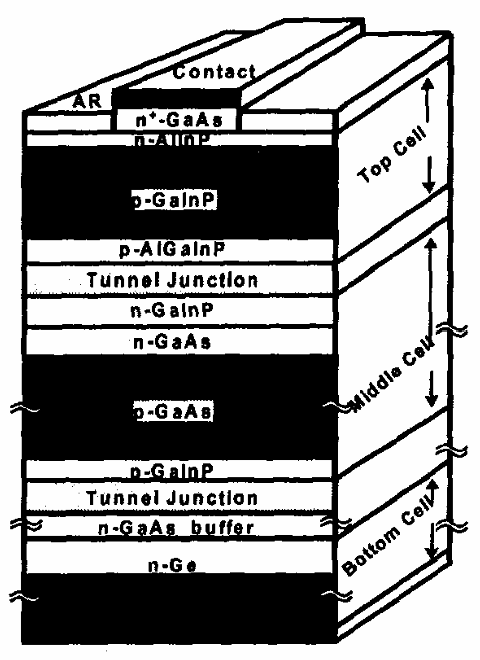
\includegraphics[width=0.70\textwidth]{figuras/figura_3_2_1_modelo_3_diodos.png}
    \caption{Circuito elétrico equivalente com três subcélulas fotovoltaicas em série.}
    \label{fig:celula}
    \vspace{2pt}\par\noindent{\footnotesize Fonte: adaptado de Cotal et al. \cite{cotal2000triplejunction}.}
\end{figure}

Os parâmetros eletroquímicos de cada subcamada semicondutora são sumarizados na Tabela~\ref{tab:subcel}.

\begin{table}[htbp]
\centering
\small
\caption{Parâmetros elétricos e papel físico de cada subcamada da célula XTJ Prime.}
\label{tab:subcel}
\begin{tabular}{p{3.2cm} r r r r p{3.4cm}}
\toprule
\textbf{Subcélula} & \textbf{$V_{oc,i}$ (V)} & \textbf{$n_i$} & \textbf{$R_{sh,i}$ ($\Omega$)} & \textbf{$J_{sc,i}$ (mA/cm$^2$)} & \textbf{Papel Físico} \\
\midrule
Topo (GaInP) & $\approx 1{,}42$ & 1,15 & 2500 & 18,00 & Limitante em início de vida. \\
Intermediária (GaAs) & $\approx 1{,}01$ & 1,15 & 3500 & 18,35 & Limitante em fim de vida. \\
Base (Ge) & $\approx 0{,}29$ & 1,75 & 200 & 26,50 & Excesso no infravermelho. \\
Célula completa & 2,720 & 4,05 & --- & 18,00 & $R_s=0{,}0914\,\Omega$ calibrado. \\
\bottomrule
\end{tabular}
\vspace{2pt}\par\noindent{\footnotesize Fonte: Cotal et al. \cite{cotal2000triplejunction} com calibração empírica do autor.}
\end{table}

A Figura~\ref{fig:fv} apresenta as curvas características I-V e P-V da string de 208 células sob diferentes patamares de temperatura orbital.

\begin{figure}[htbp]
    \centering
    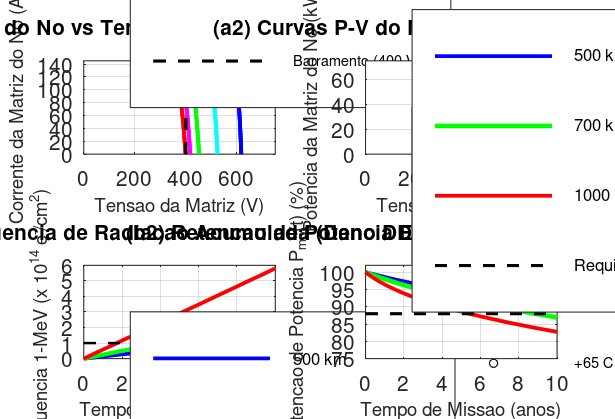
\includegraphics[width=0.85\textwidth]{figuras/figura_3_3_desempenho_termico_radiacao_am0.png}
    \caption{Curvas características I-V e P-V do gerador fotovoltaico sob espectro AM0.}
    \label{fig:fv}
    \vspace{2pt}\par\noindent{\footnotesize Fonte: elaborado pelo autor.}
\end{figure}

A caracterização paramétrica global do subsistema solar é consolidada na Tabela~\ref{tab:fv-param}.

\begin{table}[htbp]
\centering
\small
\caption{Parâmetros nominais e limites do subsistema de geração fotovoltaica.}
\label{tab:fv-param}
\begin{tabular}{p{3.0cm} p{1.2cm} p{1.8cm} p{2.2cm} p{2.0cm} p{2.4cm}}
\toprule
\textbf{Parâmetro} & \textbf{Símb.} & \textbf{Mínimo} & \textbf{Nominal} & \textbf{Máximo} & \textbf{Classificação} \\
\midrule
Irradiância solar & $G_{AM0}$ & 1322 W/m$^2$ & 1361 W/m$^2$ & 1414 W/m$^2$ & ASTM E490-22 \\
Tensões subcélula & $V_{oc,1..3}$ & --- & 1,42/1,01/0,29 V & --- & Catálogo COTS \\
Área ativa (nó) & $A_{at,no}$ & 58,95 kW & 158,19 m$^2$ & 85,52 kW & 52.416 células \\
Área total (cluster) & $A_{at,tot}$ & --- & 3163,8 m$^2$ & 1,35 MW & 20 nós orbitais \\
Tensão MPP string & $V_{mp,str}$ & 429,0 V & 453,8 V & 667,0 V & Modelo 3 diodos \\
Retenção 10 anos & EOL & 88,17\% & 90,42\% & 91,74\% & Radiação DDD \\
Potência líquida EOL & $P_{bus,EOL}$ & 46,14 kW & 49,73 kW & 54,18 kW & Regulação em 400 V \\
Ponto quente (\textit{hot spot}) & $T_{hs}$ & --- & 60,0$^\circ$C & 279,4$^\circ$C & Com e sem bypass \\
\bottomrule
\end{tabular}
\vspace{2pt}\par\noindent{\footnotesize Fonte: elaborado pelo autor.}
\end{table}

A dinâmica transitória de rastreamento de ponto de máxima potência com o algoritmo adaptativo P\&O-AP e a proteção contra pontos quentes (\textit{hot spots}) são ilustradas na Figura~\ref{fig:mppt}.

\begin{figure}[htbp]
    \centering
    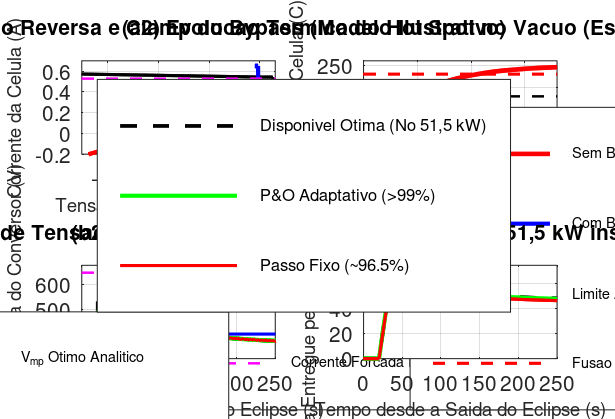
\includegraphics[width=0.85\textwidth]{figuras/figura_3_4_contingencias_hotspot_mppt.png}
    \caption{Rastreamento de máxima potência pelo algoritmo P\&O-AP e resposta térmica.}
    \label{fig:mppt}
    \vspace{2pt}\par\noindent{\footnotesize Fonte: elaborado pelo autor.}
\end{figure}

\subsection{Modelagem Térmico-Elétrica dos Semicondutores GaN e Conversores}
\label{sec:gan-dcdc}
\label{sec:conversores_estaticos}
\label{sec:magneticos}

Os estágios de comutação e os semicondutores GaN de alta frequência empregados no conversor multiportas são apresentados na Figura~\ref{fig:dab}, fundamentados na topologia proposta por Sarfi e Beik \cite{sarfi2024mwscale}.

\begin{figure}[htbp]
    \centering
    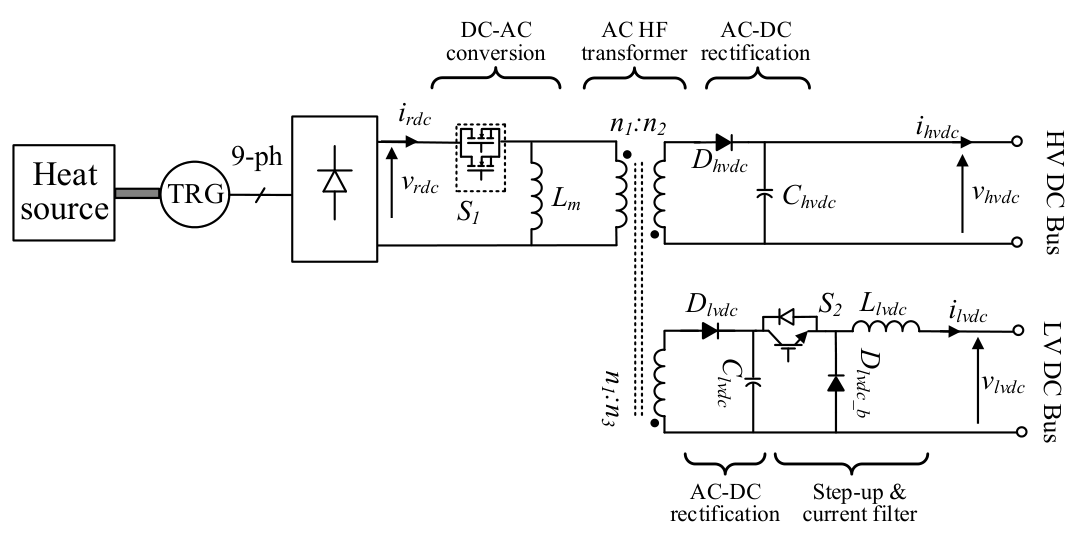
\includegraphics[width=0.80\textwidth]{figuras/figura_3_4_estagios_comutacao_DC_DC.png}
    \caption{Esquema elétrico dos estágios de comutação do conversor CC-CC primário.}
    \label{fig:dab}
    \vspace{2pt}\par\noindent{\footnotesize Fonte: adaptado de Sarfi e Beik \cite{sarfi2024mwscale}.}
\end{figure}

A resistência térmica de condução da junção para a carcaça e a impedância térmica equivalente $R_{th}$ do encapsulamento obedecem à formulação analítica:
\begin{equation}
    R_{th,eq} = R_{th,jc} + R_{th,TIM} + R_{th,base}
    \label{eq:rth_gan}
\end{equation}

A Tabela~\ref{tab:tj} analisa a temperatura de junção resultante em função do arranjo e do número de chaves empregadas.

\begin{table}[htbp]
\centering
\small
\caption{Temperatura de junção $T_j$ e margem térmica nos semicondutores GaN.}
\label{tab:tj}
\begin{tabular}{l r r r r r r}
\toprule
\textbf{Arranjo de Chaves} & \textbf{$T_j (T_c=45)$} & \textbf{$T_j (T_c=55)$} & \textbf{$T_j (T_c=60)$} & \textbf{$T_j (T_c=65)$} & \textbf{$T_{c,max}^{105}$} & \textbf{$T_{c,max}^{125}$} \\
\midrule
4 chaves (1 por ramo) & 161,0 & 178,3 & 187,0 & 195,7 & 12,7 & 24,2 \\
8 chaves (2 por ramo) & 72,4 & 83,6 & 89,2 & 94,8 & 74,2 & 92,0 \\
\bottomrule
\end{tabular}
\vspace{2pt}\par\noindent{\footnotesize Fonte: elaborado pelo autor com $R_{th}=1{,}52$~K/W (4 chaves) e $0{,}76$~K/W (8 chaves).}
\end{table}

A sensibilidade às resistências parasitas de interligação das trilhas e condutores do secundário é avaliada na Tabela~\ref{tab:sens-interlig}.

\begin{table}[htbp]
\centering
\small
\caption{Sensibilidade das perdas por condução e do rendimento às interligações.}
\label{tab:sens-interlig}
\begin{tabular}{r r r r}
\toprule
\textbf{$R_{interlig}$ (m$\Omega$)} & \textbf{$P_{cond,sec}$ (W)} & \textbf{$P_{loss,total}$ (W)} & \textbf{$\eta$ (\%)} \\
\midrule
0,000 & 211,8 & 587,4 & 97,15 \\
0,300 & 263,9 & 639,5 & 96,90 \\
0,732 & 338,9 & 714,5 & 96,55 \\
1,000 & 385,5 & 761,1 & 96,33 \\
\bottomrule
\end{tabular}
\vspace{2pt}\par\noindent{\footnotesize Fonte: elaborado pelo autor (Script~3.4).}
\end{table}

A decomposição das perdas e o perfil de rendimento eletrotérmico são ilustrados na Figura~\ref{fig:gan}.

\begin{figure}[htbp]
    \centering
    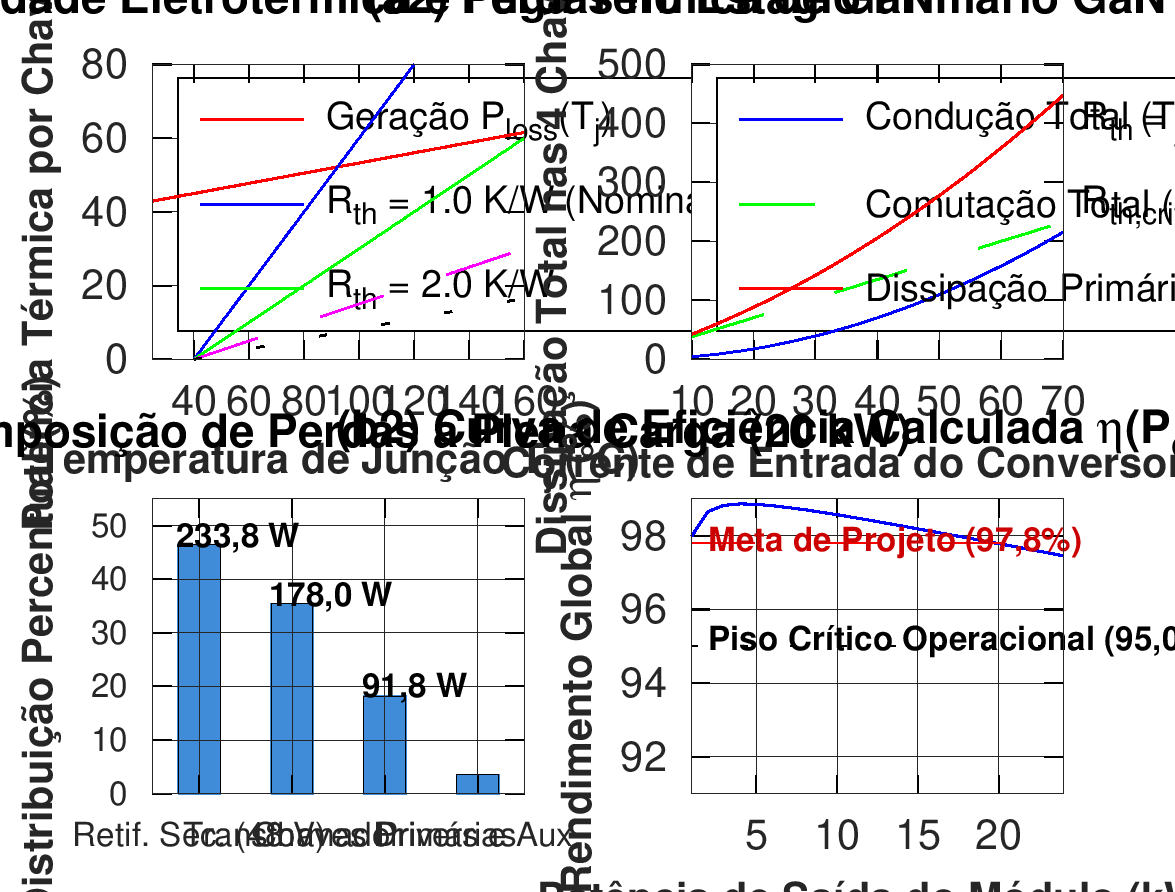
\includegraphics[width=0.85\textwidth]{figuras/figura_3_7_eletrotermica_gan_perdas.png}
    \caption{Decomposição de perdas de condução e comutação nos semicondutores GaN.}
    \label{fig:gan}
    \vspace{2pt}\par\noindent{\footnotesize Fonte: elaborado pelo autor.}
\end{figure}

A Tabela~\ref{tab:param-fontes} consolida a proveniência dos parâmetros do estágio de conversão.

\begin{table}[htbp]
\centering
\small
\caption{Origem e justificativa dos parâmetros adotados nos conversores.}
\label{tab:param-fontes}
\begin{tabular}{p{4.2cm} p{3.2cm} p{6.4cm}}
\toprule
\textbf{Parâmetro} & \textbf{Valor} & \textbf{Origem / Justificativa} \\
\midrule
$R_{th,jc}$ e $R_{DS(on)}$ do GS66516T & 0,27~K/W; 25~m$\Omega$ & Catálogo do fabricante \cite{infineon2024gs66516t} \\
$R_{th,TIM}$ & 0,85~K/W & Especificação de interface térmica \\
$R_{DS(on)}$ do retificador & 6~m$\Omega$ (máx.) & Catálogo IR HiRel \cite{infineon_ig1nt052n10r} \\
$I_d$ e tensão de bloqueio & 52~A e 100~V & Catálogo IR HiRel \cite{infineon_ig1nt052n10r} \\
Dispositivos por posição & 12 (48 no total) & Derating de corrente adotado \\
Interligações secundário & 0,732~m$\Omega$ & Resistência distribuída de barramento \\
Capacitores MLCC 2220 & $C_{ef}=11\,\mu\mathrm{F}$ & Catálogo Kyocera AVX \cite{kyocera_avx_esa} \\
ESR do banco de MLCC & 0,27~m$\Omega$ & Associação de 1364 capacitores \\
Capacitores de Tântalo & CWR Series & Qualificação espacial \cite{vishay_cwr_space} \\
\bottomrule
\end{tabular}
\vspace{2pt}\par\noindent{\footnotesize Fonte: elaborado pelo autor.}
\end{table}

A resposta em frequência da impedância de saída frente ao Critério de Middlebrook é demonstrada na Figura~\ref{fig:middlebrook}.

\begin{figure}[htbp]
    \centering
    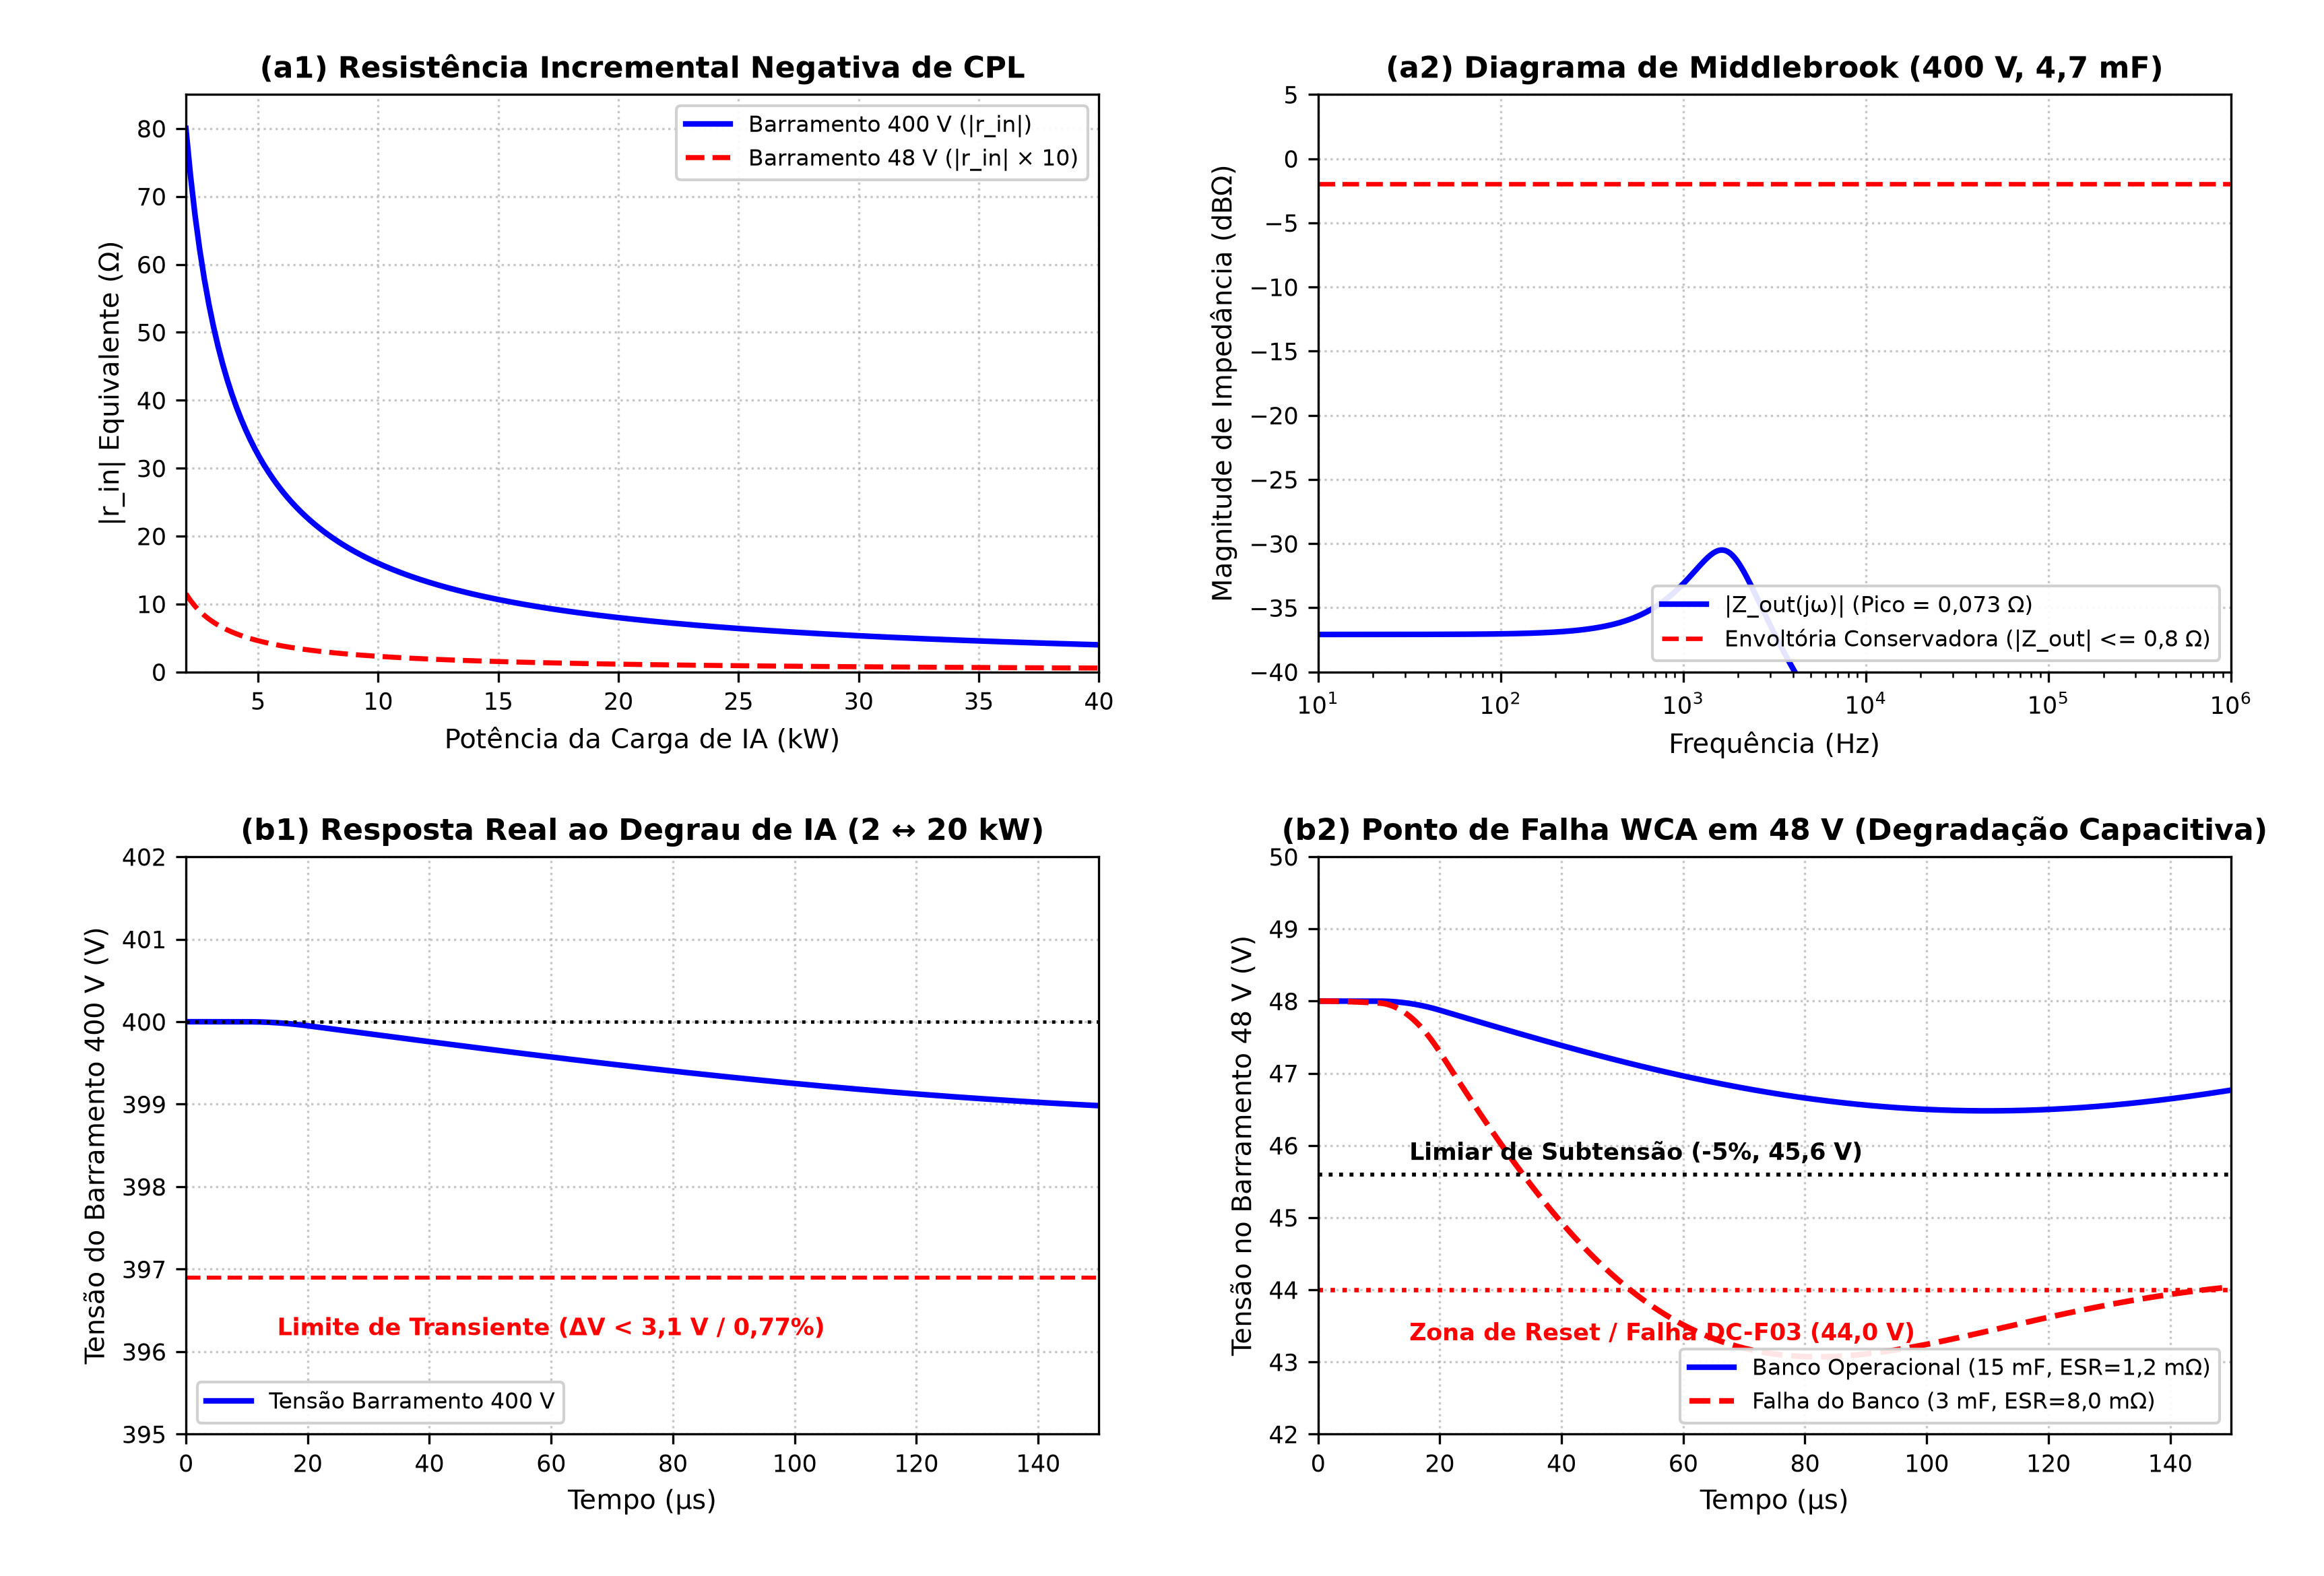
\includegraphics[width=0.85\textwidth]{figuras/figura_3_8_estabilidade_cpl_banco_capacitivo.png}
    \caption{Curvas de impedância de saída e limites de estabilidade de Middlebrook.}
    \label{fig:middlebrook}
    \vspace{2pt}\par\noindent{\footnotesize Fonte: elaborado pelo autor.}
\end{figure}

\subsection{Modelo Eletroquímico de Thevenin de 2ª Ordem e Estimador AUKF}
\label{sec:thevenin-aukf}
\label{sec:bess_eletrotermica_aukf}

O circuito elétrico equivalente de Thevenin com dois ramos RC paralelos para modelagem dos fenômenos de transferência de carga e polarização difusiva é ilustrado na Figura~\ref{fig:thevenin}.

\begin{figure}[htbp]
    \centering
    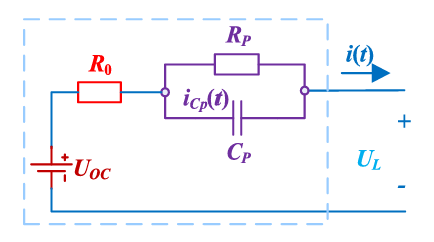
\includegraphics[width=0.60\textwidth]{figuras/figura_3_5_1_circuito_thevenin.png}
    \caption{Circuito equivalente de Thevenin de 2ª ordem para a célula de Li-ion.}
    \label{fig:thevenin}
    \vspace{2pt}\par\noindent{\footnotesize Fonte: adaptado de Feng et al. \cite{feng2022soc}.}
\end{figure}

A evolução temporal das sobretensões de polarização eletroquímica e a resposta térmica sob estresse de ciclagem são apresentadas na Figura~\ref{fig:bat-term}.

\begin{figure}[htbp]
    \centering
    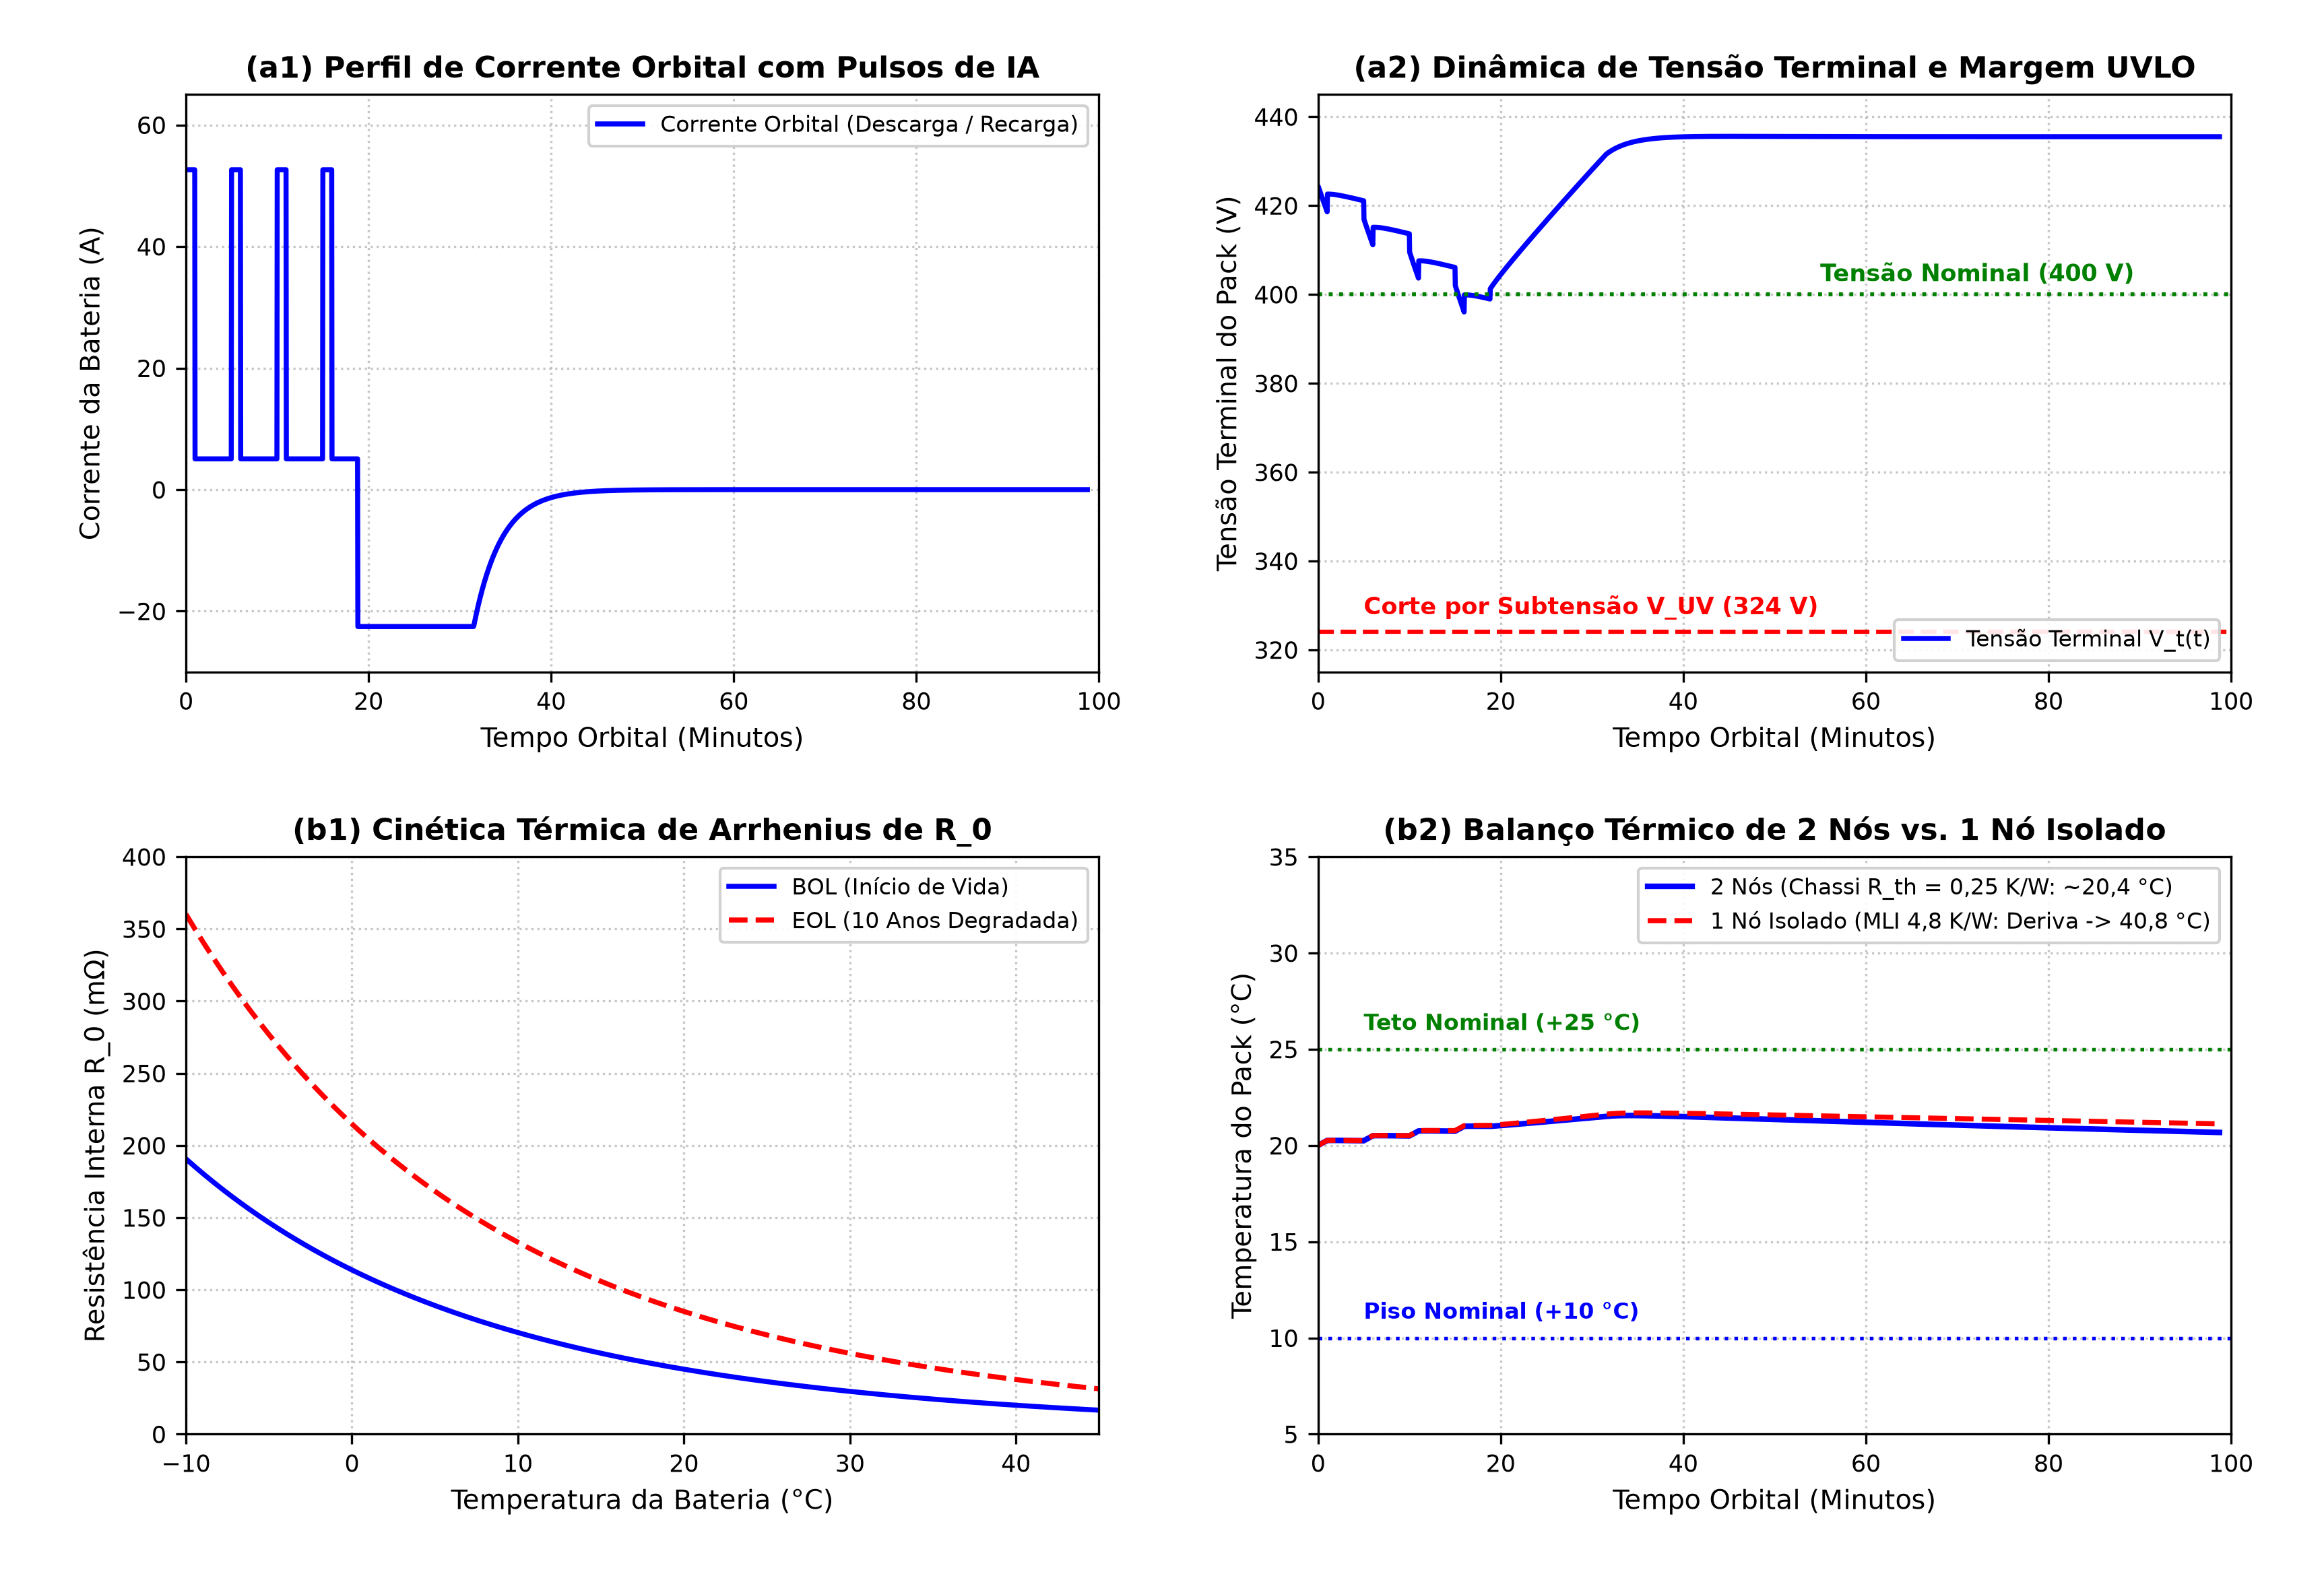
\includegraphics[width=0.85\textwidth]{figuras/figura_3_5_dinamica_dp_eletroquimica.png}
    \caption{Dinâmica de relaxamento de tensão dos ramos RC e gradiente térmico.}
    \label{fig:bat-term}
    \vspace{2pt}\par\noindent{\footnotesize Fonte: elaborado pelo autor.}
\end{figure}

A Tabela~\ref{tab:bess-orb} sumariza as métricas de recarga e dissipação térmica no pack ao longo da órbita.

\begin{table}[htbp]
\centering
\small
\caption{Métricas eletrotérmicas do pack BESS sob diferentes temperaturas de string.}
\label{tab:bess-orb}
\begin{tabular}{l r r r r r r r}
\toprule
\textbf{Cenário} & \textbf{$P_{chg}$ (kW)} & \textbf{$SoC_{min}$ (\%)} & \textbf{$SoC_{fim}$ (\%)} & \textbf{$\bar{I}_{ecl}$ (A)} & \textbf{$\bar{P}_{J}$ (W)} & \textbf{$T_{pico}$ ($^\circ$C)} & \textbf{$T_{eq}$ ($^\circ$C)} \\
\midrule
$85^\circ$C & 4,98 & 27,89 & 99,67 & 51,0 & 62,7 & 25,9 & 23,8 \\
$65^\circ$C & 6,57 & 28,18 & 99,96 & 50,9 & 66,0 & 26,1 & 24,2 \\
$28^\circ$C & 11,02 & 28,21 & 99,99 & 50,9 & 70,3 & 26,5 & 24,8 \\
\bottomrule
\end{tabular}
\vspace{2pt}\par\noindent{\footnotesize Fonte: elaborado pelo autor.}
\end{table}

A arquitetura computacional do Filtro de Kalman Adaptativo Unscented (AUKF) livre de derivadas \cite{JulierUhlmann2004,feng2022soc} e o rastreamento em malha fechada do estado de carga sob degraus de potência são apresentados na Figura~\ref{fig:aukf-dupla}.

\begin{figure}[htbp]
    \centering
    \begin{minipage}{0.48\textwidth}
        \centering
        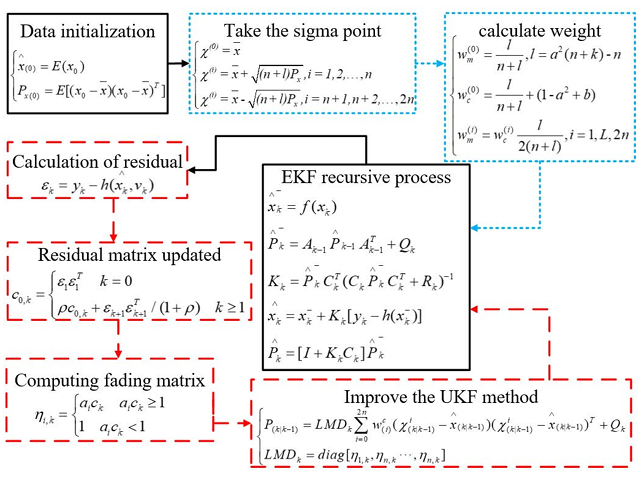
\includegraphics[width=\linewidth]{figuras/figura_3_5_3_estrutura_algoritmo.png}
        \caption{Estrutura do estimador AUKF.}
        \label{fig:aukf-alg}
    \end{minipage}\hfill
    \begin{minipage}{0.48\textwidth}
        \centering
        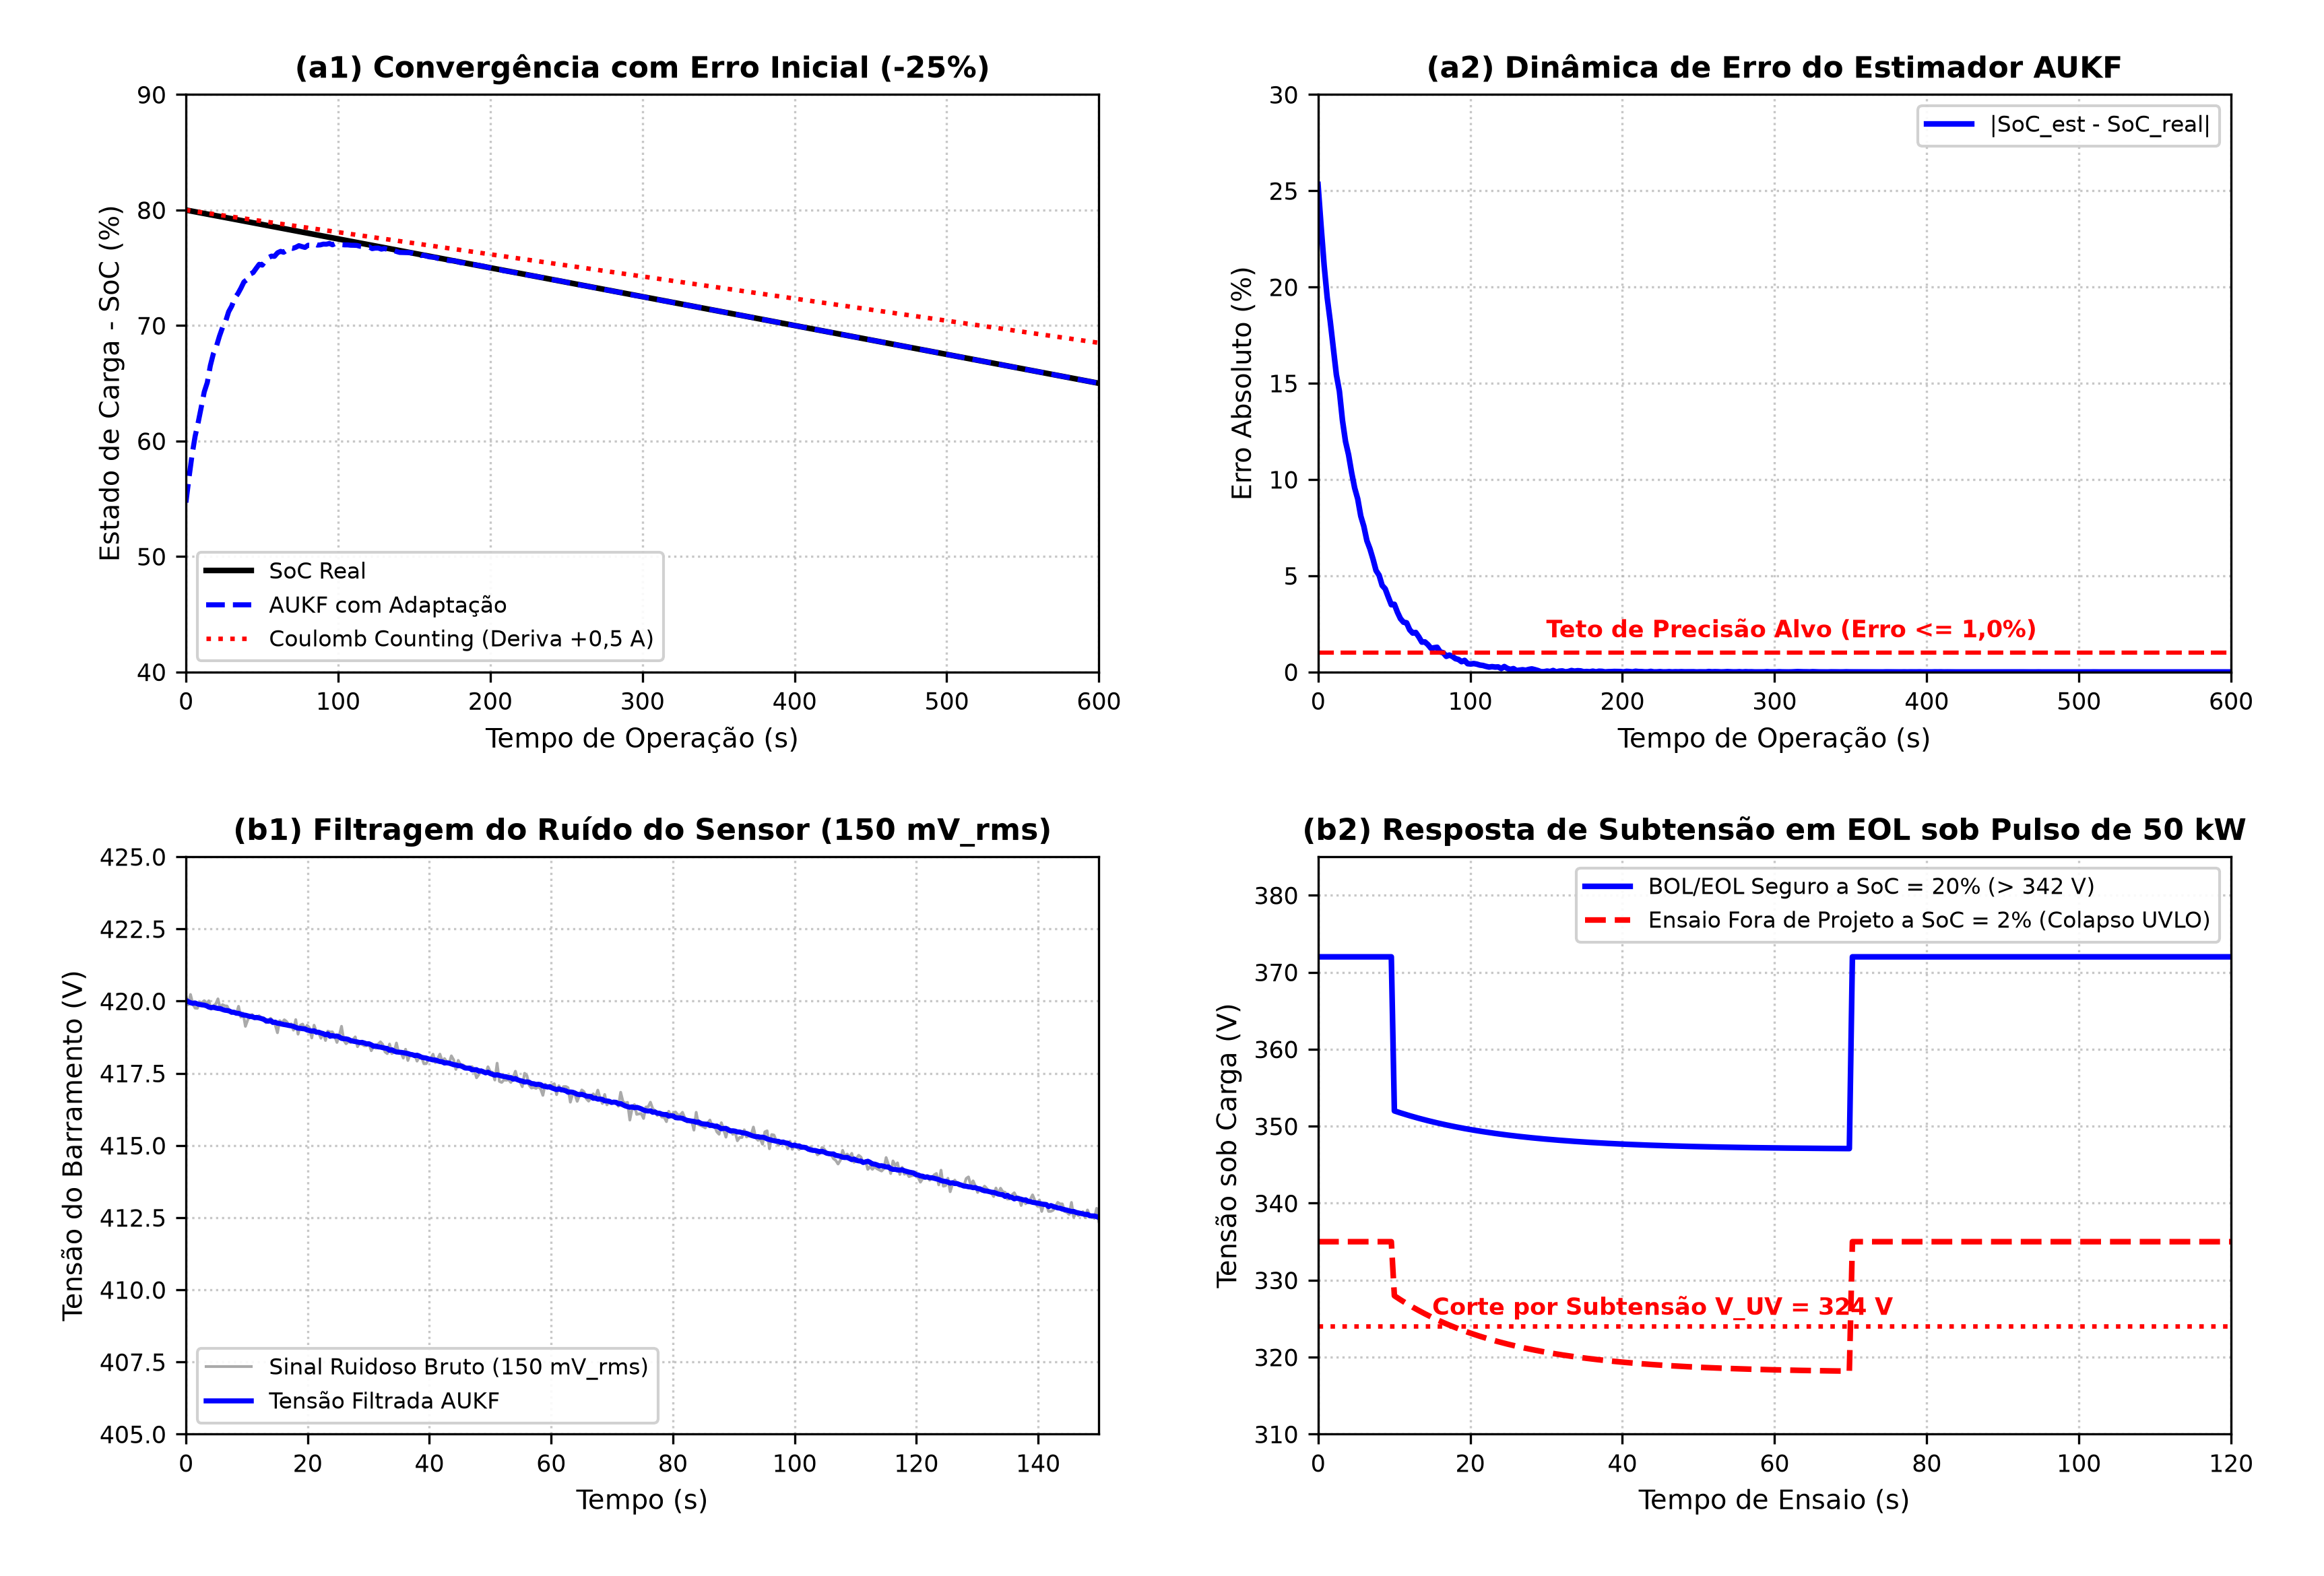
\includegraphics[width=\linewidth]{figuras/figura_3_6_convergencia_aukf_estresse.png}
        \caption{Convergência sob degrau de carga.}
        \label{fig:aukf-convergencia}
        \label{fig:aukf-dupla}
    \end{minipage}
    \vspace{2pt}\par\noindent{\footnotesize Fonte: elaborado pelo autor com base em \cite{JulierUhlmann2004,feng2022soc}.}
\end{figure}